\documentclass[../main.tex]{subfiles}

\begin{document}

\renewcommand{\thefootnote}{\roman{footnote}}

\subsection{Anaconda}

Anaconda\footnote{https://www.anaconda.com/} es una distribución de software que incluye diversas aplicaciones y librerías, entre las cuales están Python, Spyder y Jupyter. Tiene como objetivo facilitar la administración e implementación de librerías y paquetes, además de simplificar la gestión de entornos. Es la plataforma más completa para trabajar con Data Science.

\begin{figure}[h]
	\centering
	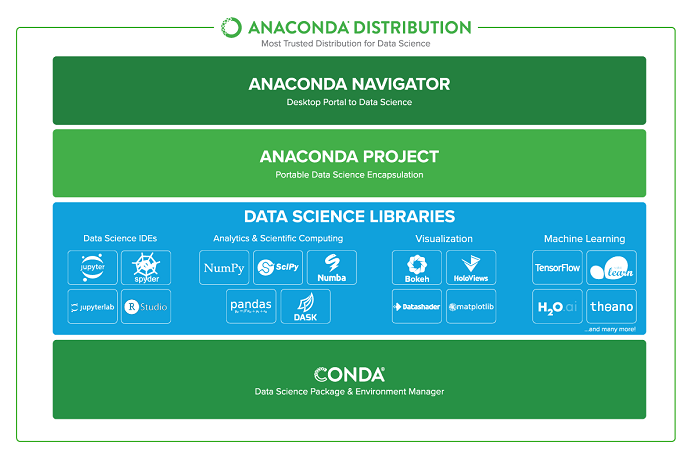
\includegraphics[width=0.7\textwidth]{../images/anaconda-distribution.png}
	\caption{Elementos principales de Anaconda. \cite{anaconda2017figure}}
\end{figure}

Se clasifica en cuatro partes: Anaconda Navigator, Anaconda Project, Conda y las librerías de ciencia de datos.

\subsection{Spyder}
Spyder\footnote{https://www.spyder-ide.org/} es un entorno de programación para Python gratuito y de código abierto. Está escrito en Python. Su diseño está enfocado para uso científico y análisis de datos.

\subsection{Jupyter}

Jupyter Notebook\footnote{https://jupyter.org/} es una aplicación web para crear y compartir documentos computacionales. Ofrece un manejo sencillo, y está centrado en los documentos. Los cuadernos pueden contener código y datos.

JupyterLab es una evolución del anterior. Su interfaz permite a los usuarios configurar y organizar flujos de trabajo en ciencia de datos. Posee un diseño modular que invita a realizar ampliaciones que mejoren su funcionalidad.

\subsection{Python}

Python\footnote{https://www.python.org/} es un lenguaje de propósito general creado a finales de los años 80 por Guido van Rossum.

Entre sus características destacadas están:

\begin{itemize}
	
	\item Es interpretado.
	
	\item Es dinámico. Las variables pueden ser de cualquier tipo, ya que de base todas las variables son objetos.
	
	\item Es multiplataforma.
	
	\item Es de código abierto.
	
\end{itemize}

En los últimos años ha aumentado su popularidad en el desarrollo de software para la ingeniería de datos y \textit{machine learning}.

\subsubsection{PyPDF2}

PyPDF2\footnote{https://github.com/py-pdf/PyPDF2} es una librería de Python cuyo función es manejar las páginas de los archivos PDF. También puede añadir y modificar datos, recuperar texto y metadatos.

\subsubsection{pdfminer.six}

Pdfminer.six\footnote{https://github.com/pdfminer/pdfminer.six} es un paquete de Python que sirve para extraer información de documentos en formato PDF.


\end{document}
